\documentclass[tikz]{standalone}
% B A C D E
% D C A E B
% rauzy induction after step 1
% A C D E
% C A E D
% rauzy induction after step 1'
% A C    D E
% C A    E D
\begin{document}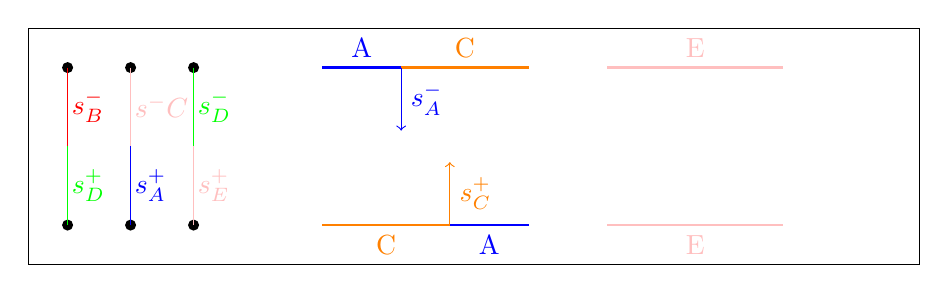
\begin{tikzpicture}

\draw (-.5, -1.5) rectangle (10.82,1.5);

\coordinate (t0) at (1,1);
\coordinate (t1) at (3.23606797749979, 1);
\coordinate (t2) at (4.23606797749979, 1);
\coordinate (t3) at (5.85410196624968, 1);
\coordinate (tt3) at (6.85410196624968, 1);
\coordinate (t4) at (9.09016994374947, 1);
\coordinate (t5) at (11.32623792124926, 1);

\coordinate (b0) at (1,-1);
\coordinate (b1) at (3.23606797749979, -1);
\coordinate (b2) at (4.85410196624968, -1);
\coordinate (b3) at (5.85410196624968, -1);
\coordinate (bb3) at (6.85410196624968, -1);
\coordinate (b4) at (9.09016994374947, -1);
\coordinate (b5) at (11.32623792124926, -1);

\draw[thick,blue] (t1) -- node[above] {A} (t2);
\draw[thick,orange] (t2) -- node[above] {C} (t3);
\draw[thick,pink] (tt3) -- node[above] {E} (t4);
j
\draw[thick,orange] (b1) -- node[below] {C} (b2);
\draw[thick,blue] (b2) -- node[below] {A} (b3);
\draw[thick,pink] (bb3) -- node[below] {E} (b4);

\draw[->,orange] (b2) -- node[right] {$s^+_C$} +(0,0.8);

\draw[->,blue] (t2) -- node[right] {$s^-_A$} +(0,-0.8);


\fill[black] (0,-1) circle (2pt);
\fill[black] (0,1) circle (2pt);
\draw[green] (0,-1) -- node[right=-2] {$s^+_D$} (0,0);
\draw[red] (0,1) -- node[right=-2] {$s^-_B$} (0,0);

\fill[black] (.8,-1) circle (2pt);
\fill[black] (.8,1) circle (2pt);
\draw[blue] (.8,-1) -- node[right=-2] {$s^+_A$} (.8,0);
\draw[pink] (.8,1) -- node[right=-2] {$s^-C$} (.8,0);

\fill[black] (1.6,-1) circle (2pt);
\fill[black] (1.6,1) circle (2pt);
\draw[pink] (1.6,-1) -- node[right=-2] {$s^+_E$} (1.6,0);
\draw[green] (1.6,1) -- node[right=-2] {$s^-_D$} (1.6,0);

\end{tikzpicture}\end{document}
